\documentclass{article}
\usepackage{graphicx}

\title{Imaginarily Complex; Really Simple}
\author{Rohan Dhillon}

\begin{document}

\maketitle
You’ve probably heard of complex numbers before—good old formulas like $i=\sqrt{-1}$, $z=a+bi$, and $|z|=a^2+b^2$ hopefully ring a bell (if they don’t, this article might be pretty confusing). But did you know that complex numbers have a lot of use beyond just the confusion of high school students? In fact they’re used in everything from counting sums to describing our universe. 

But we’re getting ahead of ourselves. First we really need to understand complex numbers at the fundamental level—and I mean very fundamental. Why did we come up with them anyway? In the 1500s, we still didn’t know how to solve a cubic equation in full. The primary problem was that square roots of negative numbers kept popping up everywhere—at the time, no one had conceived of an imaginary number. However, an Italian mathematician by the name of Gerolamo Cardano decided to let $\sqrt{-1}$ exist as a concept. When he did, the solutions to a depressed cubic, a special type of cubic whose $x^2$ coefficient is $0$, fell into place immediately. 
\begin{center}
    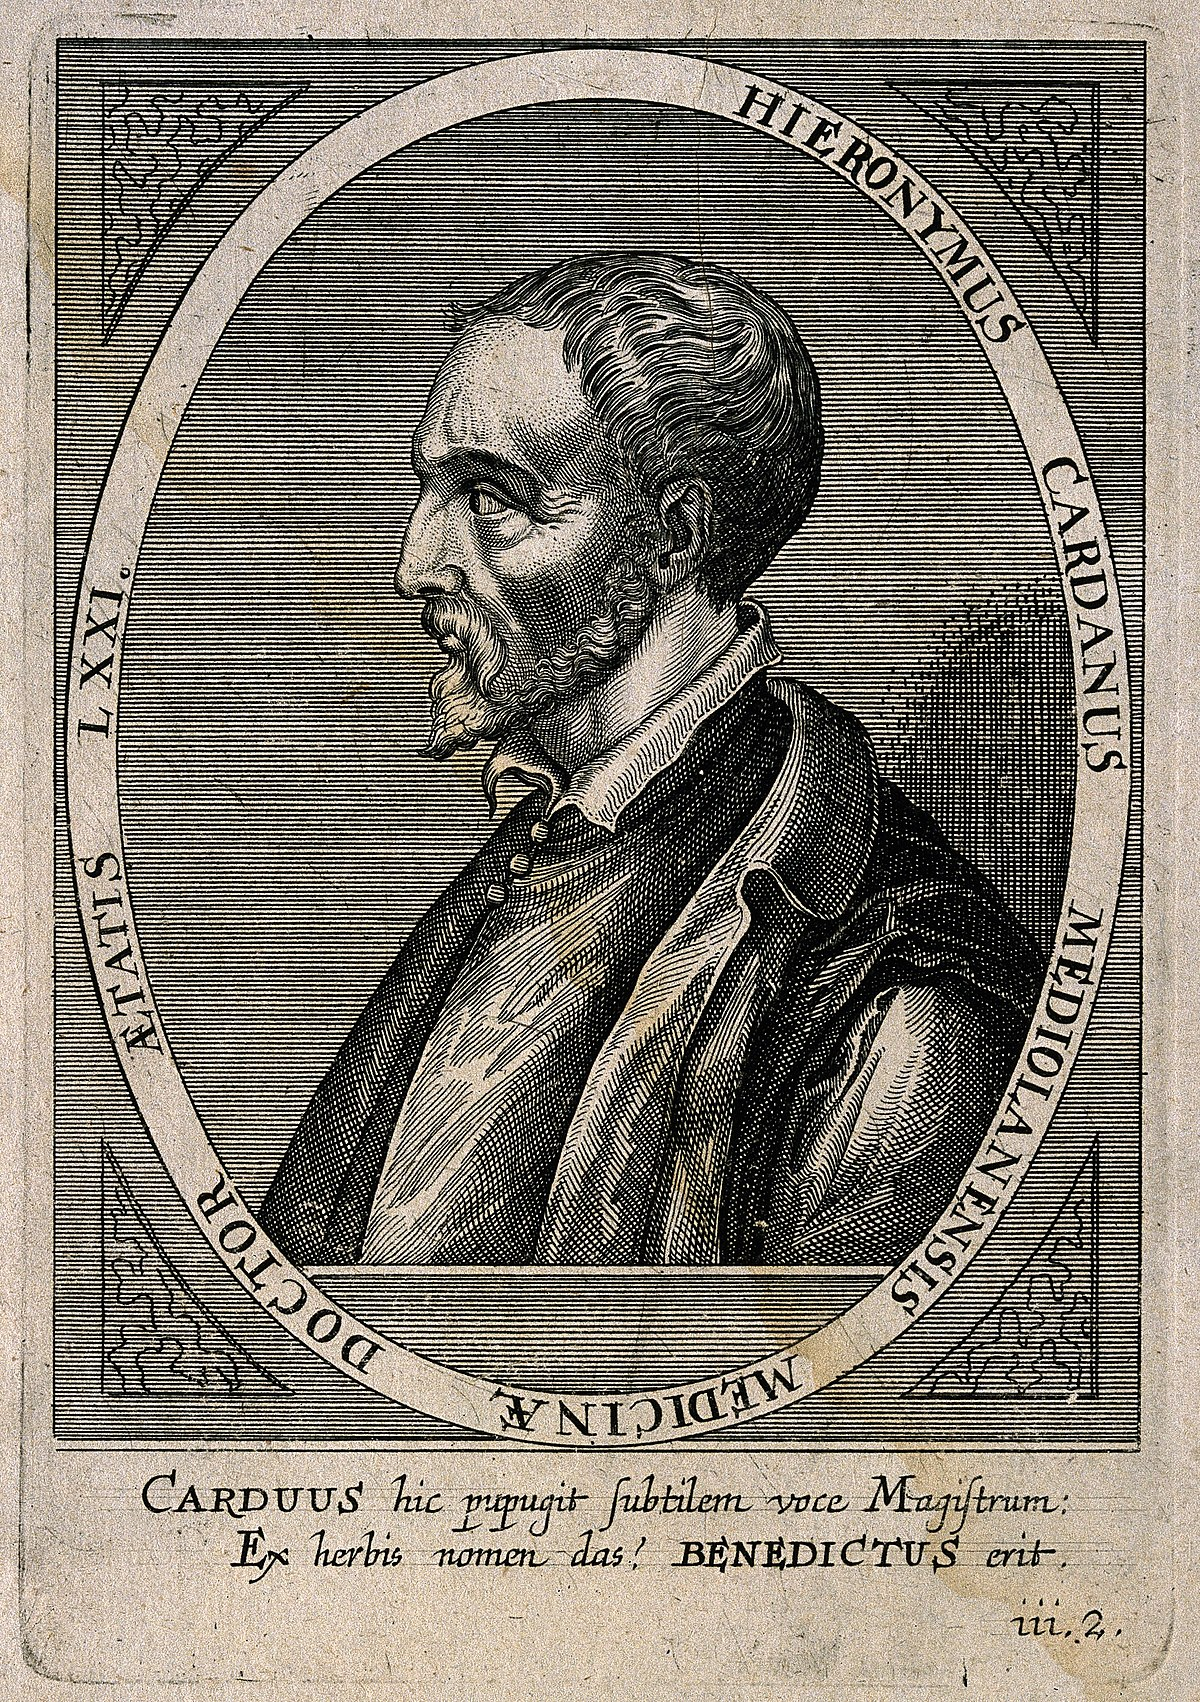
\includegraphics[scale=0.1]{images/gerolamo.jpg}
\end{center}
And then, some centuries later on, we came up with the Fundamental Theorem of Algebra which states that any polynomial equation of degree $n$ has $n$ roots (some can be repeated). But then what are the roots of, say, $x^7=1$? Here’s where we have to think of complex numbers differently. Rather than defining $z=a+bi$, let’s define it as $z=(r,\theta)$, where $r=|z|$ and $\theta$  is the angle the complex number makes with the positive $x$-axis counterclockwise. (This definition is akin to treating a complex number as a point in polar coordinates). 

With this idea in mind, we have a very useful formula for the multiplication of complex numbers (which we won’t prove): DeMoivre’s Formula: $pq=(r_pr_q,\theta_p+\theta_q)$. Basically, we multiply magnitudes and add angles. So if we take powers we should get $z^n=(r^n,n\theta)$. 
\begin{center}
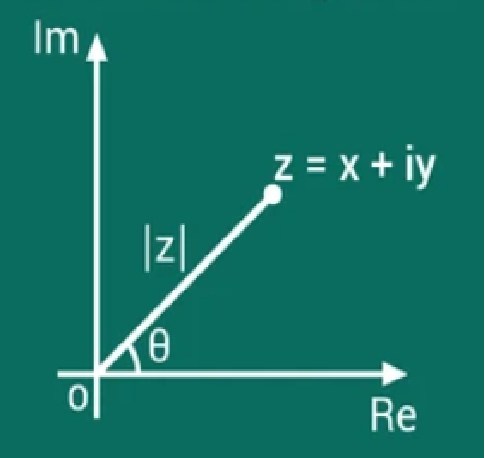
\includegraphics[scale=0.8]{images/complex1.png}
\end{center}
One is also a complex number, however, with $1=(1,0)=(1,2\pi)=(1,4\pi)$.... So we’re looking for all complex numbers x such that $x^7=(r^7,7\theta)=(1,2\pi k)$. Well, since $r$ is always a positive number, $r=1$ and for , we can just divide by $7$ to get $\theta=\frac{2\pi k}{7}$. Thus, we have our seven solutions as promised. These seven solutions are called the seventh roots of unity. In general, all of the solutions to $x^n=1$ are called $n$th roots of unity. 

So complex numbers are made to solve algebraic (usually polynomial) equations. But in how many ways can we really use this fact? It’s not like some counting problem could be solved with complex numbers right? Well…that’s the funny thing. There’s a few important problems that can. One of the more famous one (at least in math competition circles) is one variant of the following:

\textit{Suppose we choose a subset of numbers from {1,2,...,100}. What is the probability they sum to a multiple of 5?} The first thing we need to do is create a \textit{generating function}. These essentially turn finding the numbers of ways to count something into finding the coefficients of a polynomial. For our problem, the generating function is 
$$g(x)=(x+1)(x^2+1)...(x^{100}+1).$$ 
Each term $x^n+1$ says that we can either choose $n$ or $1$. When we multiply everything out, the coefficient of each term tells us the number of ways to get it. For example, the constant term is $1=1x^0$ meaning there is one way to get a sum of $0$. Meanwhile, the $x^{5050}$ coefficient is also $1$, meaning there’s one way to get a sum of $5050$. 

Okay, so all we need to do is find the sum of the coefficients of $x^5,x^{10},x^{15},...,x^{5050}$. Hmmmm…that doesn’t seem easy…unless we use roots of unity. Let the five roots of unity to $x^5=1$ be $z_0=1, z_1=(1,72), z_2=(1,144), z_3=(1,216), z_4=(1,288)$. Then, note that all of these roots of unity sum to $0$…and their squares sum to $0$…and their cubes sum to $0$…and their fourth powers too! But thankfully, since their fifth powers must all be $1$, their fifth powers sum to $5$. Aha! If we take $g(z_0)+g(z_2)+...+g(z_4)$, we get a nonzero sum only on fifth powers. This is exactly what we want! So all we need to do is find the above sum and divide it by $5$! But…how do we do that? 
	
Let’s take one root of unity—say $z_1$ for simplicity (note that taking $1$ will just give us $2^100$). Then, we want $(z_1+1)(z_1^2+1)(z_1^{100}+1)=[(z_1+1)(z_1^5+1)]^20$ since after taking the root to the sixth power, we arrive back at the original root. All we need to do is find the thing inside of the square brackets. Now, we turn away from polar notation and back into our $a+bi$ form. Doing this gives us $z_1=\cos 72+i\sin 72, z_2=\cos 144+i\sin 144$, and so on. 
\begin{center}
    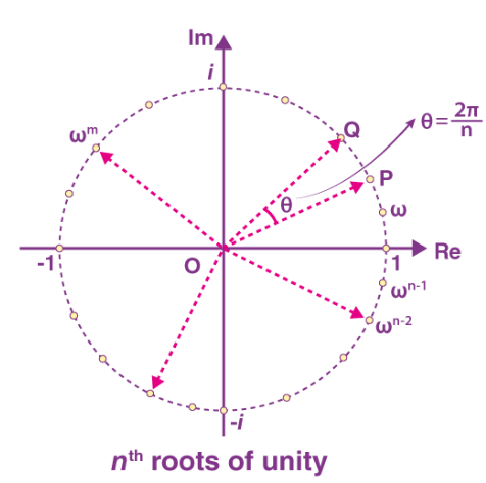
\includegraphics[scale=0.7]{images/root1.png}
\end{center}
But now notice that $z_4=\overline{z_1}, z_3=\overline{z_2}$, and adding the real number $1$ to those quantities won't change anything. Thus what we really want is 
$z_1\overline{z_1}z_2\overline{z_2}\cdot 2=|z_1|^2|z_2|^2\cdot 2$. 

This is just 
\begin{align*}
 & [(1+\cos 72)^2+\sin^2 72)  \cdot   \\
 & ((1+\cos 144)^2+\sin^2 144]  = \\
 & [2+2\cos 72][2+2\cos 144]  = \\
 & 4(1+\cos 72+\cos 144+\cos 72 \cos 144)
\end{align*}


From here the only way to really proceed is to know that $\cos 144=-\cos 36$, $\cos 18=\frac{1+\sqrt5}{2}$, and $\cos 2\theta=2\cos^2 \theta -1$. Plugging all of these things in and slogging through the arithmetic we get that our expression is $2$—exactly. Then, our $20$th power expression is $2^20$, and our answer is simply $\frac{4\cdot 2^{20}+2^{100}}{5}$ ways — a little more than exactly a fifth. 
And there you have it—imaginary numbers solving a very \emph{real} problem (okay, maybe not that real but you get the point). I hope that you’ve gotten a sense of just how powerful this topic is—and that was just the introduction. Complex numbers have a special place in geometry problems, where they simplify arithmetic, and in quantum mechanics, where they quite literally define how particles behave. So there you have it: complex numbers—conceived in a mathematician's head, but known by the universe for 13.8 billion years. 
\begin{center}
    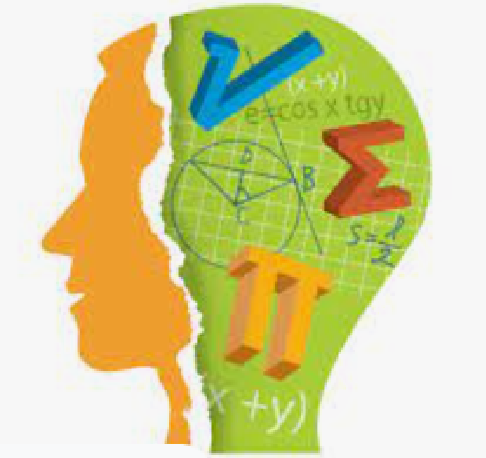
\includegraphics[scale=0.7]{images/root2.png}
\end{center}
\end{document}